%% rnaastex.cls is the classfile used for Research Notes. It is derived
%% from aastex61.cls with a few tweaks to allow for the unique format required.

%% Better is to use the "RNAAS" style option in AASTeX v6.2
%% (01/08/18)
\documentclass[RNAAS, modern]{aastex62}

%% Define new commands here
\newcommand\latex{La\TeX}

%    Make Scientific Notation
\providecommand{\e}[1]{\ensuremath{\times 10^{#1}}}

% make the word Kepler italicized
\newcommand{\Kepler}{\textsl{Kepler}\xspace}

\begin{document}

\title{Using Flare Rates to Search for Stellar Activity Cycles}

%% Note that the corresponding author command and emails has to come
%% before everything else. Also place all the emails in the \email
%% command instead of using multiple \email calls.

\correspondingauthor{Matthew T. Scoggins}
\email{scoggim@wwu.edu}

\author{Matthew Scoggins}
\affiliation{Department of Physics \& Astronomy, Western Washington University, 516 High St., Bellingham, WA 98225, USA}

\author{James. R. A. Davenport}
\altaffiliation{DIRAC Fellow}
\affiliation{Department of Astronomy, University of Washington, Seattle, WA 98195, USA}

\author{Kevin R. Covey}
\affiliation{Department of Physics \& Astronomy, Western Washington University, 516 High St., Bellingham, WA 98225, USA}


%% Note that RNAAS manuscripts DO NOT have abstracts.
%% See the online documentation for the full list of available subject
%% keywords and the rules for their use.
% \keywords{stars: cycles, flares}
%%%% Keywords are OUT (2019), instead we should use the UAT http://astrothesaurus.org with these 2: Flare stars, Solar cycle

%% Start the main body of the article. If no sections in the 
%% research note leave the \section call blank to make the title.
\section{} 



Measuring the prevalence and duration of stellar activity cycles gives key insight into the origin of stellar magnetic dynamos. The canonical activity cycle is the Sun's, which lasts approximately 11 years. Assuming this represents a typical stellar cycle, years to decades of observations are required to detect cyclic magnetic activity in other stars. Currently, activity cycles for other stars are traced through either precise integrated flux measurements \citep{kopp2016}, chromospheric emission line monitoring campaigns \citep{duncan1991}, or starspot tracking \citep{messina2002,montet2017}. However, all these approaches have challenges: integrated flux variations require photometric precision not possible for most stars, spectroscopic monitoring campaigns are expensive, and starspots statistics are difficult to gather for distant stars and may not reliably track activity ``butterfly diagrams'' \citep{morris2019}.



However, solar activity data suggests that flares may be a good measure for tracking magnetic activity cycles. 
Flares are eruptions that emit across the EM spectrum \citep[e.g. see][]{hawley2003}, produced during magnetic re-connection events. The rate that flares are produced is therefore directly related to the star's surface magnetic field strength. Additionally, flares are easily detectable for distant stars (e.g. up to a kpc away), and can be surveyed for many stars simultaneously using wide-field photometric surveys. Thus, flares are a promising avenue for tracing stellar activity cycles; encouragingly, the Sun's flare rate varies by a factor of ∼10 between solar “maximum” and “minimum” \citep[e.g.][]{veronig2002, aschwanden2012}. 



Here we briefly explore this idea, searching for variations in the rate of white light flares from stars in the Kepler mission \citep{borucki2010}. Kepler provides up to 4 year long, nearly continuous optical light curves. Although we don't expect to observe entire cycles in Kepler light curves, we search for coherent variations in flare rate that may indicate these stars are undergoing activity cycles. We examined a sample of 347 flare stars from \citet{davenport2019}, which were selected as having measured photometric rotation periods from Kepler, at least 100 candidate flare events, and at least 10 flare events with energies above the estimated 68\% detection recovery floor of their automated pipeline.

 
We search for coherent variations in flare activity by computing the fractional luminosity emitted in flares, $L_{fl}/L_{Kp} \equiv \xi_{tot}/t_{exp}$, defined by \citet{lurie2015}. Here $\xi_{tot}$ is the sum of the ``equivalent duration'' for each flare event, which can be simply converted to energies by multiplying by the stellar Luminosity \citep{huntwalker2012}, and $t_{exp}$ is the total exposure time of the observation. For every star we compute $\log L_{fl}/L_{Kp}$ over each quarter of Kepler data individually. We then use a Markov Chain Monte Carlo (MCMC) routine to fit a linear model to the time dependence of $\log L_{fl}/L_{Kp}$, seeking stars with statistically significant slopes (i.e. changes in flare activity level).
 
 

\begin{figure}
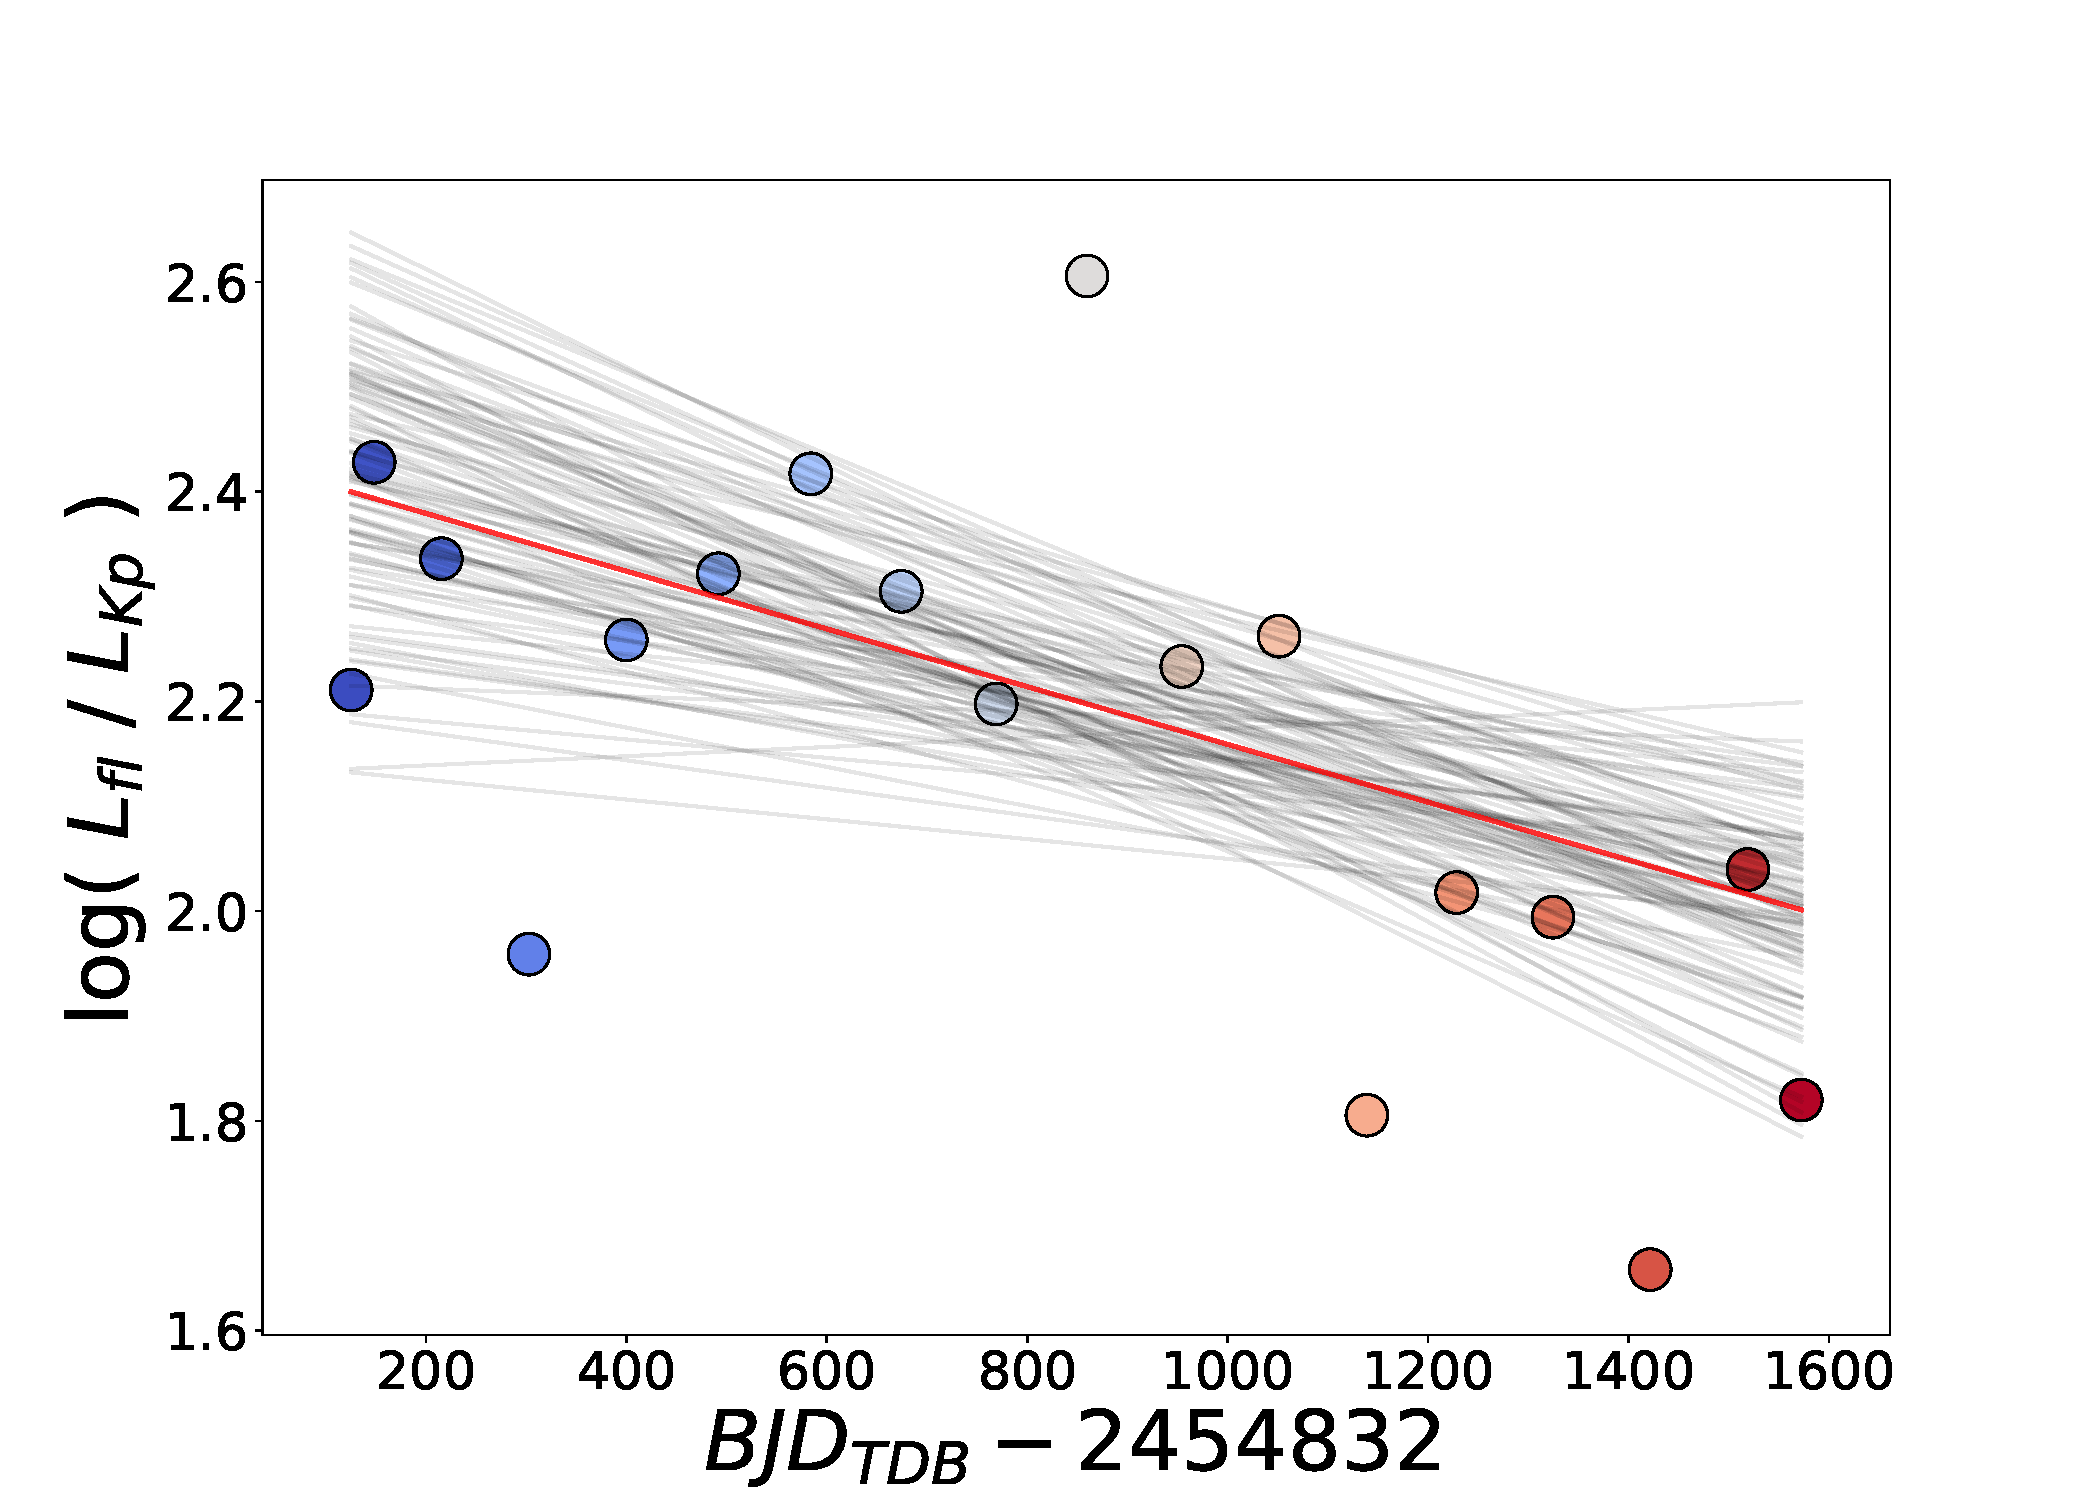
\includegraphics[width=.49\textwidth]{008507979_frac_lum.pdf}
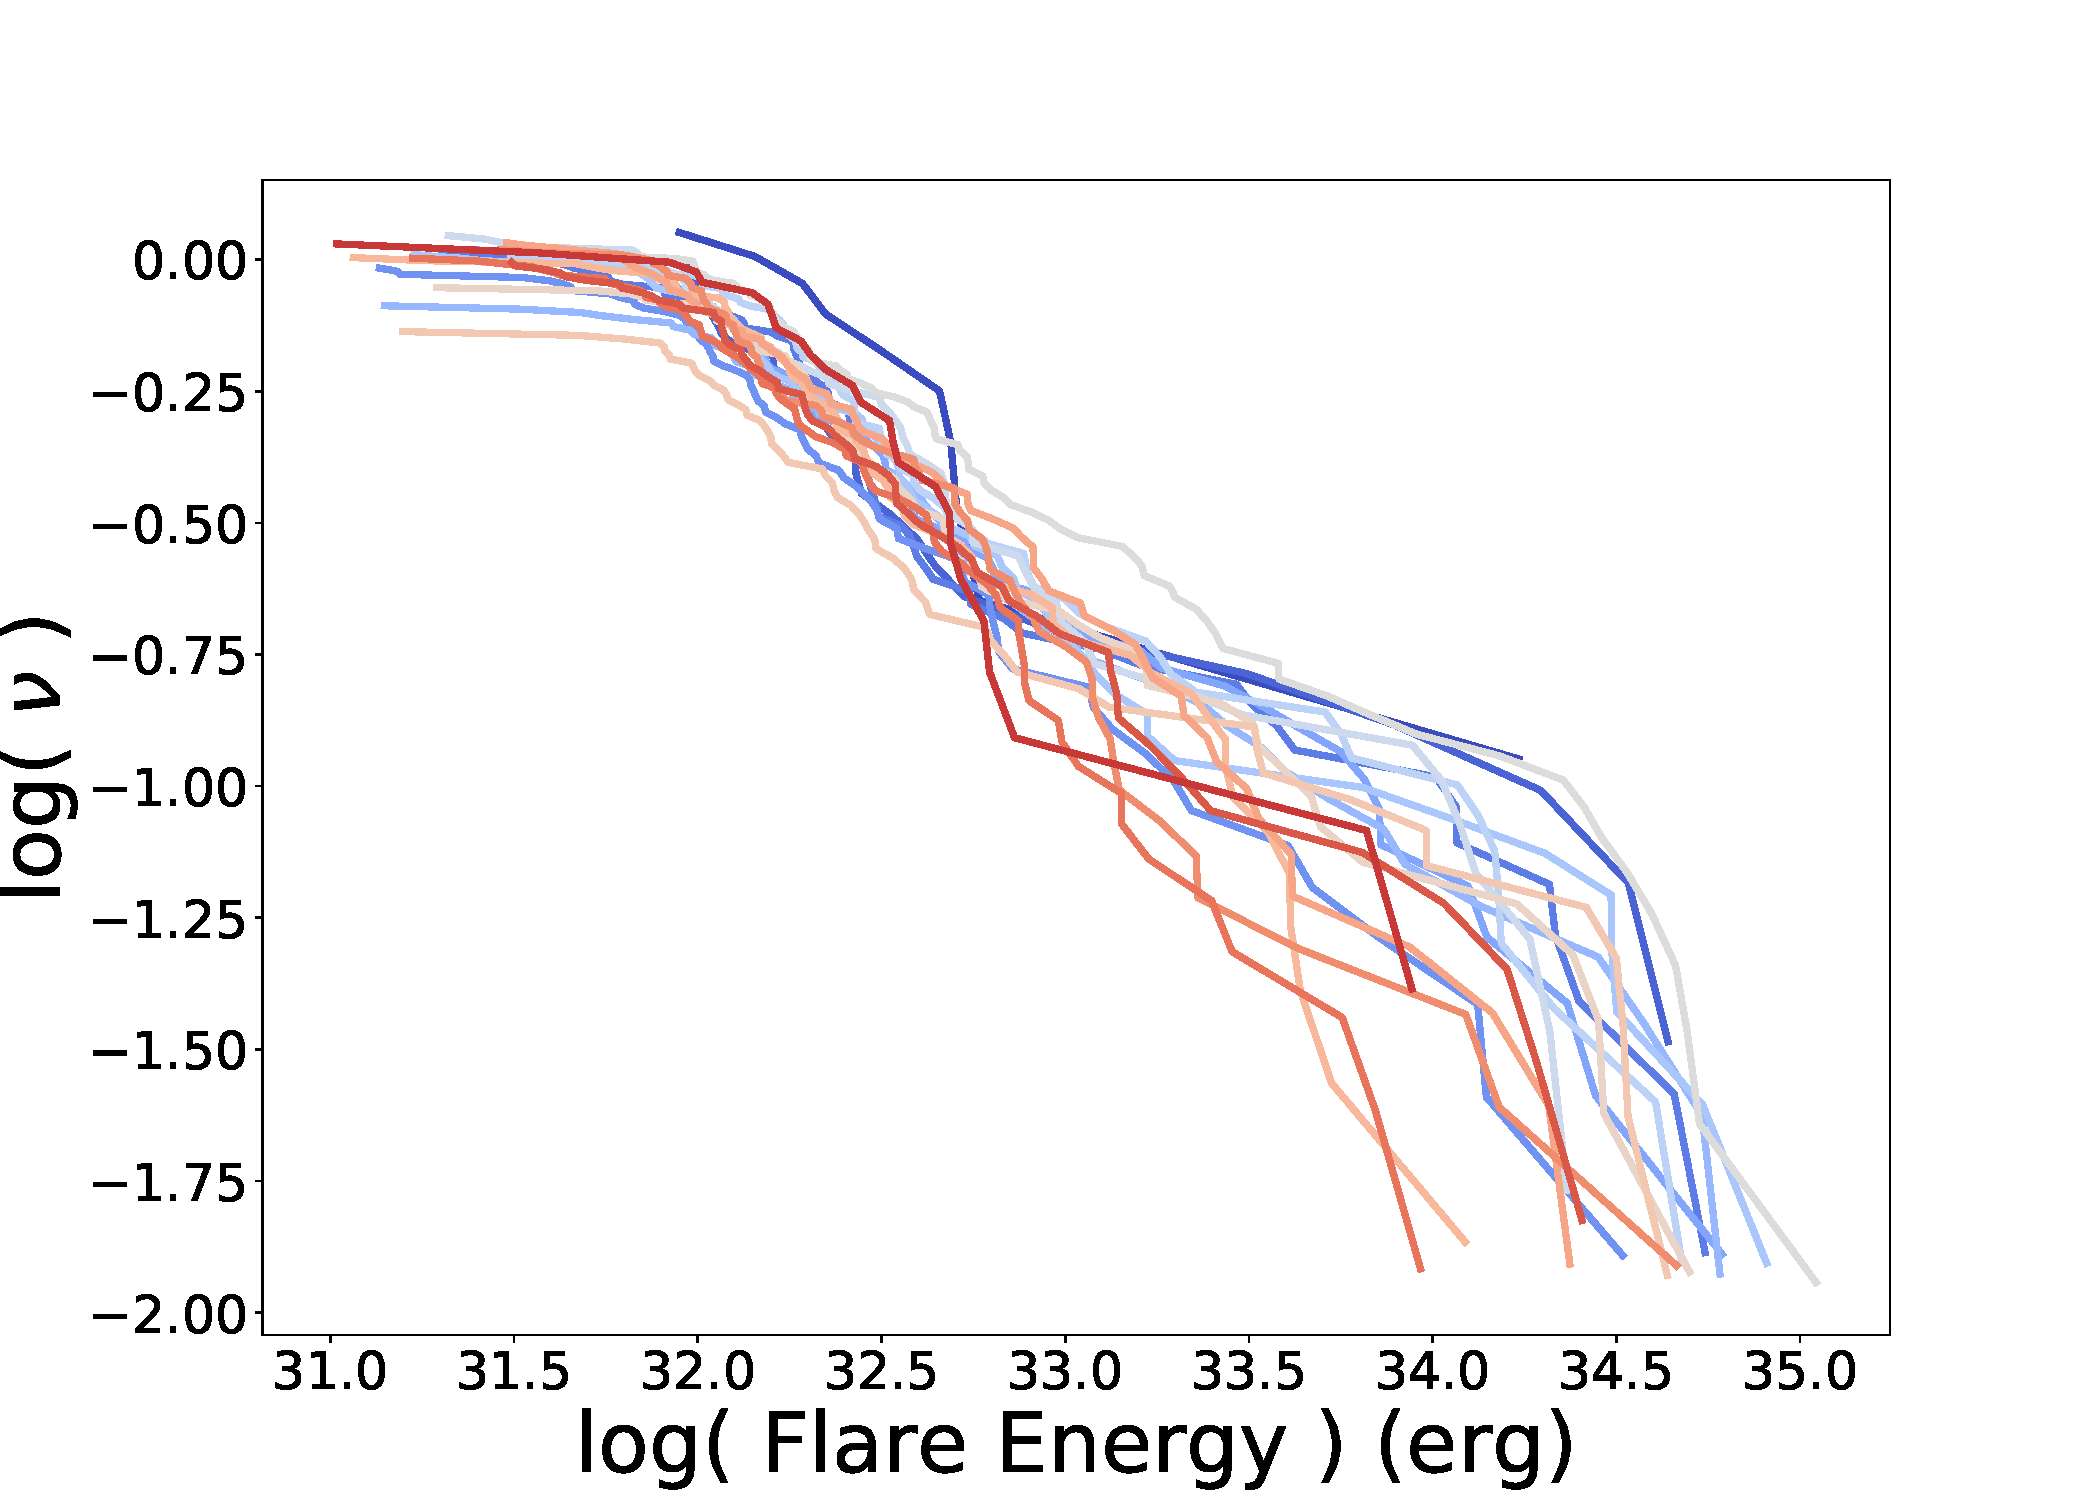
\includegraphics[width=.49\textwidth]{008507979_evf.pdf}
\caption{
{\bf Left:} Our candidate star, KIC 8507979, shows a slow decline of $\sim$0.5 dex in fractional flare luminosity ($L_{fl}/L_{Kp}$) over 4 years. Points are color-coded blue-to-red according to the observing Quarter throughout the Kepler mission. Uncertainties in $L_{fl}/L_{Kp}$ are smaller than the symbol sizes, as explored by \citet{lurie2015}. Our best MCMC linear fit is shown (red line), with 100 draws from the posterior distribution (grey lines).
{\bf Right:} Cumulative flare frequency distribution for each quarter showing a gradient in flare rate over time. Line color for each quarter matches points in the left panel.
}
\label{fig1}
\end{figure}


In Figure \ref{fig1} we show our best candidate for flare activity variation, KIC 8507979, a dM3e with a rotation period of 1.2 days. This star emits on average 0.82 flare(s) per day with energy over $10^{32}$ erg over the 18 Kepler quarters. A decline in flare activity is seen, with a MCMC best fit of 
 $\log L_{fl}/L_{Kp} =(-9.96\pm3.94)\e{-2} \times t_{years} + 2.43\pm0.11$.



We also show in Figure \ref{fig1} the flare frequency distribution for KIC 8507979 for each quarter of Kepler data. This is the standard figure for flare activity \citep[e.g.][]{lme1976,davenport2019}, and shows a negative power law correlation between flare energy and cumulative occurrence frequency. The decline in flare activity found with $L_{fl}/L_{Kp}$ can be seen in this figure as well, visible here as a color gradient, and is most noticeable for large flares with log(flare energy) $\geq$ 33.0.


While the flare census from KIC 8507979's Kepler light curve doesn't show unambiguous evidence for a stellar activity cycle, the variation of $\sim$0.1 dex per year is consistent with cyclic behavior over a decade or longer timescale. Longer baseline flare monitoring is needed to confirm cyclical behavior.
Fortunately, Sectors 14 and 15 from the Transiting Exoplanet Survey Satellite \citep[TESS;][]{tess} will revisit the original Kepler field with comparable light curve sampling (30 min cadence here). Though TESS has a considerably smaller aperture than Kepler (i.e. shallower photometric depth), bright flares will still be detectable with TESS for many of the active Kepler stars. This Kepler--TESS overlap will provide an initial 10-year observing baseline, made even more powerful for long term flare monitoring by the proposed multi-year TESS Extended Mission. We anticipate flare activity variations will therefore be an exciting new avenue for discovering and characterizing stellar magnetic activity cycles.

\software{Python, IPython \citep{ipython}, NumPy \citep{numpy}, Matplotlib \citep{matplotlib}, SciPy \citep{scipy}, Pandas \citep{pandas}, emcee \citep{emcee}}

\acknowledgements

JRAD acknowledges support from the DIRAC Institute in the Department of Astronomy at the University of Washington. The DIRAC Institute is supported through generous gifts from the Charles and Lisa Simonyi Fund for Arts and Sciences, and the Washington Research Foundation. 

This research was supported by the National Aeronautics and Space Administration (NASA) under grants 80NSSC19K0375 from the TESS Cycle 1 Guest Investigator Program, and 80NSSC18K1660 issued through the NNH17ZDA001N Astrophysics Data Analysis Program.



\bibliography{citations.bib}

\end{document}

